\documentclass[border=3pt]{standalone}
\usepackage{tikz}
\usetikzlibrary{arrows.meta,calc,positioning}
\tikzset{pin/.style={-{Stealth[length=5pt]}},
  blk/.style={draw, thick, font=\sffamily\small, align=center}}
\begin{document}
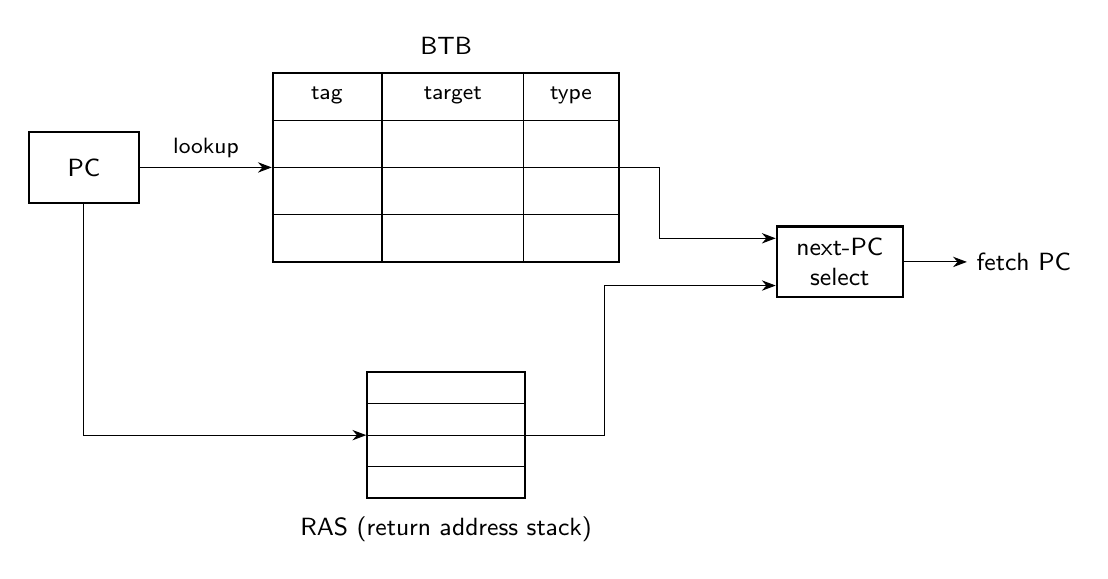
\begin{tikzpicture}[font=\sffamily\small]
  \node[blk, minimum width=14mm, minimum height=9mm] (pc) at (0,0) {PC};
  % BTB table: tag | target | type columns
  \node[blk, minimum width=44mm, minimum height=24mm] (btb) at (4.6,0) {};
  \node[font=\sffamily\small, above=1mm of btb.north] {BTB};
  \draw ($(btb.north west)+(14mm,0)$) -- ($(btb.south west)+(14mm,0)$);
  \draw ($(btb.north west)+(32mm,0)$) -- ($(btb.south west)+(32mm,0)$);
  \foreach \y in {-6,0,6}{\draw ($(btb.west)+(0,\y mm)$) -- ($(btb.east)+(0,\y mm)$);}
  \node[font=\sffamily\footnotesize] at ($(btb.north west)+(7mm,-3mm)$)  {tag};
  \node[font=\sffamily\footnotesize] at ($(btb.north west)+(23mm,-3mm)$) {target};
  \node[font=\sffamily\footnotesize] at ($(btb.north west)+(38mm,-3mm)$) {type};
  \draw[pin] (pc.east) -- node[above, font=\sffamily\footnotesize]{lookup} (btb.west);
  % RAS
  \node[blk, minimum width=20mm, minimum height=16mm] (ras) at (4.6,-3.4) {};
  \node[font=\sffamily\small, below=1mm of ras.south] {RAS (return address stack)};
  \foreach \y in {-4,0,4}{\draw ($(ras.west)+(0,\y mm)$) -- ($(ras.east)+(0,\y mm)$);}
  \draw[pin] (pc.south) |- (ras.west);
  % next-PC mux
  \node[blk, minimum width=16mm, minimum height=9mm] (mux) at (9.6,-1.2) {next-PC\\select};
  \draw[pin] (btb.east) -- ++(5mm,0) |- ($(mux.west)+(0,3mm)$);
  \draw[pin] (ras.east) -- ++(10mm,0) |- ($(mux.west)+(0,-3mm)$);
  \draw[pin] (mux.east) -- ++(8mm,0) node[right]{fetch PC};
\end{tikzpicture}
\end{document}
